\chapter{Преглед резултата}

Приликом израде  рада развијено је софтверско окружење којим су се тестирали различити приступи решавању задатог проблема. Пре свега овде се мисли на различите мере сличности које су тестиране.  Основна мера квалитета решења је \textbf{просечна позиција} тачног одговора у листи свих одговора. Што је просечна позиција нижа тј. ближа 1 то се решење сматра квалитетнијим, при чему се тежи да стандардна девијација буде што мања.
Поред просечне позиције, битне карактеристике решења су брзина рада и меморијски захтеви.

Свака од тестираних мера сличности има своје параметре који су у мањој или већој мери осетљиви на одабир корака  у предпроцесирању. Обзиром да се ради о алгоритму моделовања тема, у зависноти од мере, биће потребан различит број тема и итерација како би се постигло оптимално решење. Због тога је било неопходно испитати за сваки меру посебно како који кораци предпроцеситрања утичу и  које вредности параметара алгоритма моделовања тема су оптималне за ту меру.  

Прво тестирање решења проблема вршено је на скупу од 360 питања и 360 одговора преузетих са сајта \textit{stackexchange.com}. 


\section{Утицај броја тема и броја итерација на просечну позицију}

Обзором на то да расподела тема по документима, у мањој или већој мери, утиче на свако од тестираним мера, број тема представља битан параметар. Са малим бројем тема а на основу предложених мера, јако је тешко рангирати одговоре. Разлог томе је што ће се теме дефинисати према областима којима се баве документи. Према томе документи из исте области имаће сличне расподеле по темама а самим тим и приближно исту удаљеност од тестног документа односно питања. Због тога је неопходно да број тема буде довољно велики како би се овај проблем заобиша. 

Међутим, није добро узети ни превелики број тема. У том случају сви документи ће имати сличну расподелу по темама па ће и одстојање од тестног документа бити приближно исто. Ово директно утиче на просечну позицију сводећи је на број који је једнак $[\frac{brojDokumenata}{2}]$. Овако нешто може се видети на следећем графику \footnote{Ово тестирања  је рађено на самом почетку и то на полазном скупу од 150 докумената. Тај скуп је подскуп скупа на коме су вршена сва остала тестирања} :

		\begin{figure}[H]
    \centering
   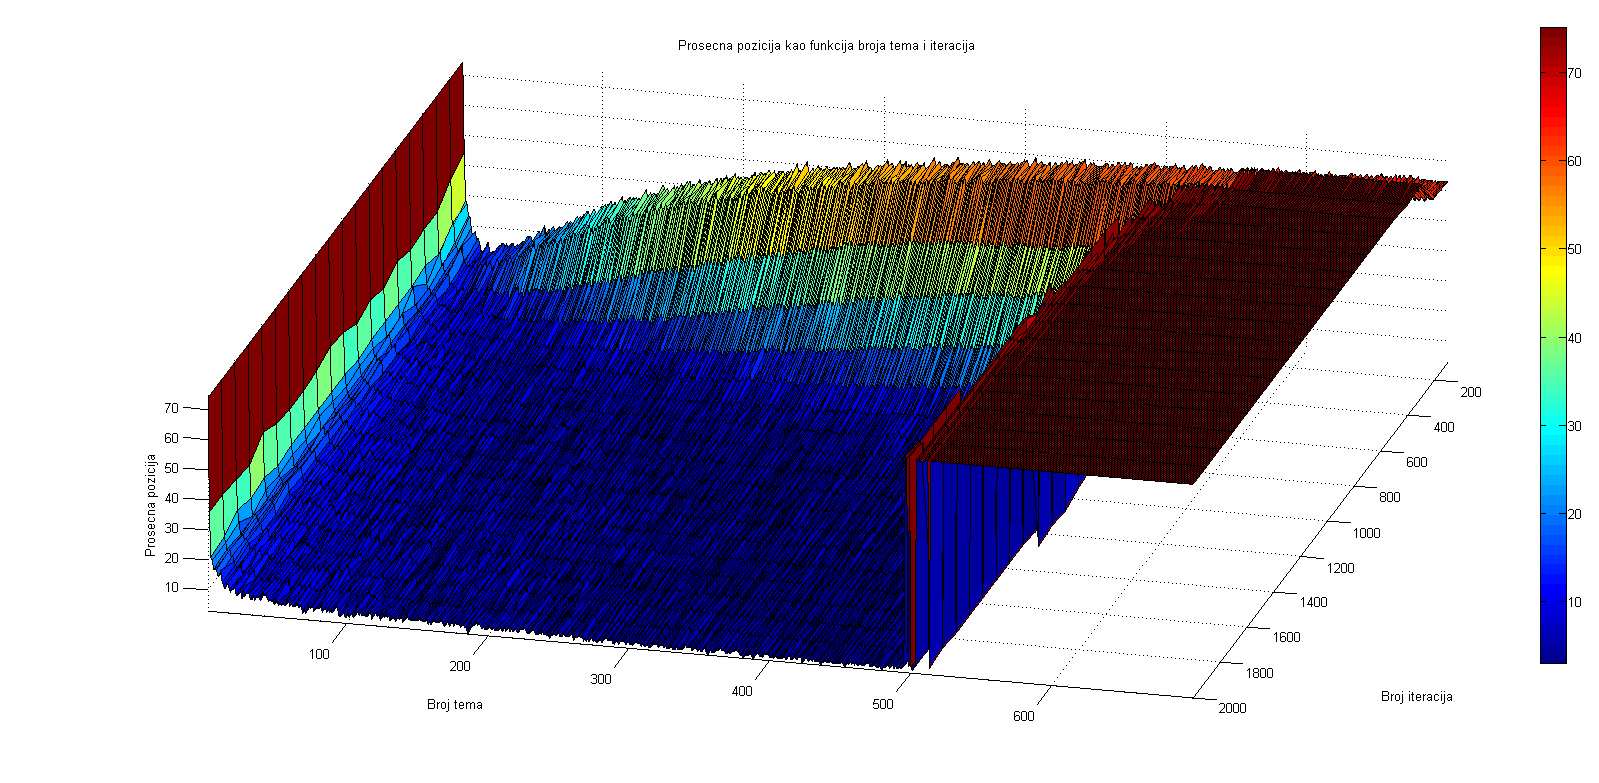
\includegraphics[scale=0.3]{./Slike/cutoff.png} 
	\caption{Зависност просечне позиције од броја тема и броја итерација}
	\label{fig:slika1}
\end{figure}


Прелаз на просечну позицију $[\frac{brojDokumenata}{2}$ ( у конкретном случају 74 јер је број докумената 150 ) је прилично груб. Разлог томе је што нису тестиране све вредности броја итерација него свака 100-та. Како je за потребе рада било довољно  уочити да се број тема не може бесконачно повећавати, ова појава даље није испитивана.


\section{Утицај корака предпроцесирања на просечну позицију}

Предпроцесирањем се \textbf{трансформише} текст улазних података како би био погоднији за обраду. Сама природа проблема намеће неке кораке предпроцесирања као неопходне. У њих спадају :

\begin{itemize}
\item превођење свих слова текста у мала слова - ова трансформација је неопходна како се не би  реч написана почетним великим словом и иста реч написана почетним малим словом третирали као две различите речи
\item уклањање HTML ознака - обзиром на порекло података, поред корисног текста, у документима се налазе и HTML ознаке које, са аспетка овог проблема, немају никаквог значаја.
\item уклањање свих неалфанумеричких карактера - овом трансформацијом се уклањају знакови интерпукције и специјални знакови који нису битни за решење овог проблема
\item уклањање често коришћених речи - оне не носе тематско значење, честе су у свим документима и представљју оптерећење при обради
\end{itemize}

Ове трансформације су се увек укључивале, без обзира на  меру сличности. Поред њих, додате су и стеминг, лемитизација и синоним трансформације у различитим комбинацијама. 


\subsection{Резултати без додатних трансформација}

Улазни подаци - и питања и одговори - трансформисани преко три описана корака предпроцесирања и то у редоследу :  превођење свих слова текста у мала слова, уклањање HTML ознака и уклањање често коришћених речи.

	\subsubsection{Косинусна сличност}
Уколико се за меру сличности одабере \textbf{косинусна} мера, просечна позиција тачног одговора директно зависи од параметара модела тј. од броја тема и броја итерација. Та зависност се може приказати следећим графиком. ( слика 5.1)
		\begin{figure}[H]
    \centering
   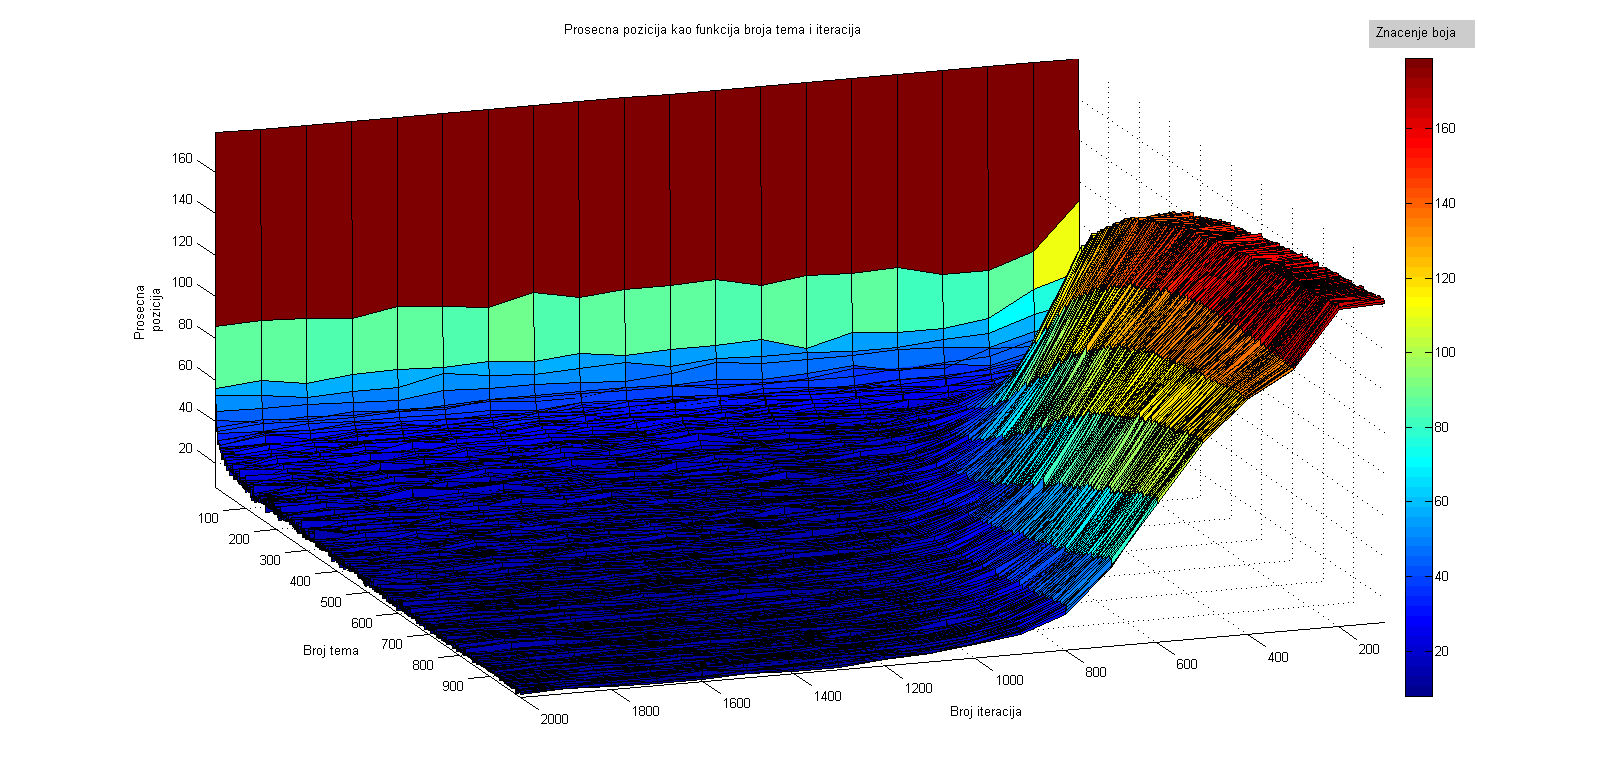
\includegraphics[scale=0.3]{./Slike/noStemNoSyn.png} 
	\caption{Зависност просечне позиције од броја тема и броја итерација}
	\label{fig:slika1}
\end{figure}

Минимална просечна позиција је \textbf{8} и добија се при више различитих комбинација параметара. Неке од комбинација су приказане у следећој табели

\begin{center}
\captionof{table}{Утицај броја тема и итерација на просечну позицију тачног одговора}
\begin{tabular}{|c|c|}
\hline
Број итерација & Број тема \\
\hline\hline
1200 & 693 \\
1400 & 756 \\
1400 & 820 \\
\hline
\end{tabular}

\end{center}

	\subsubsection{Мерење сличности према лексичкој и тематској сличности}
	
Уколико се за меру сличности одабере мера  \textbf{лексичке и теметске} сличности, просечна позиција такође директно зависи од параметра модела. Обзиром на временску и просторну сложеност ове мере, нису испитиване све могућности за параметре модела. График зависности просечне позиције од броја тема и итерација дат јена следећој слици (слика 5.2)

		\begin{figure}[H]
    \centering
   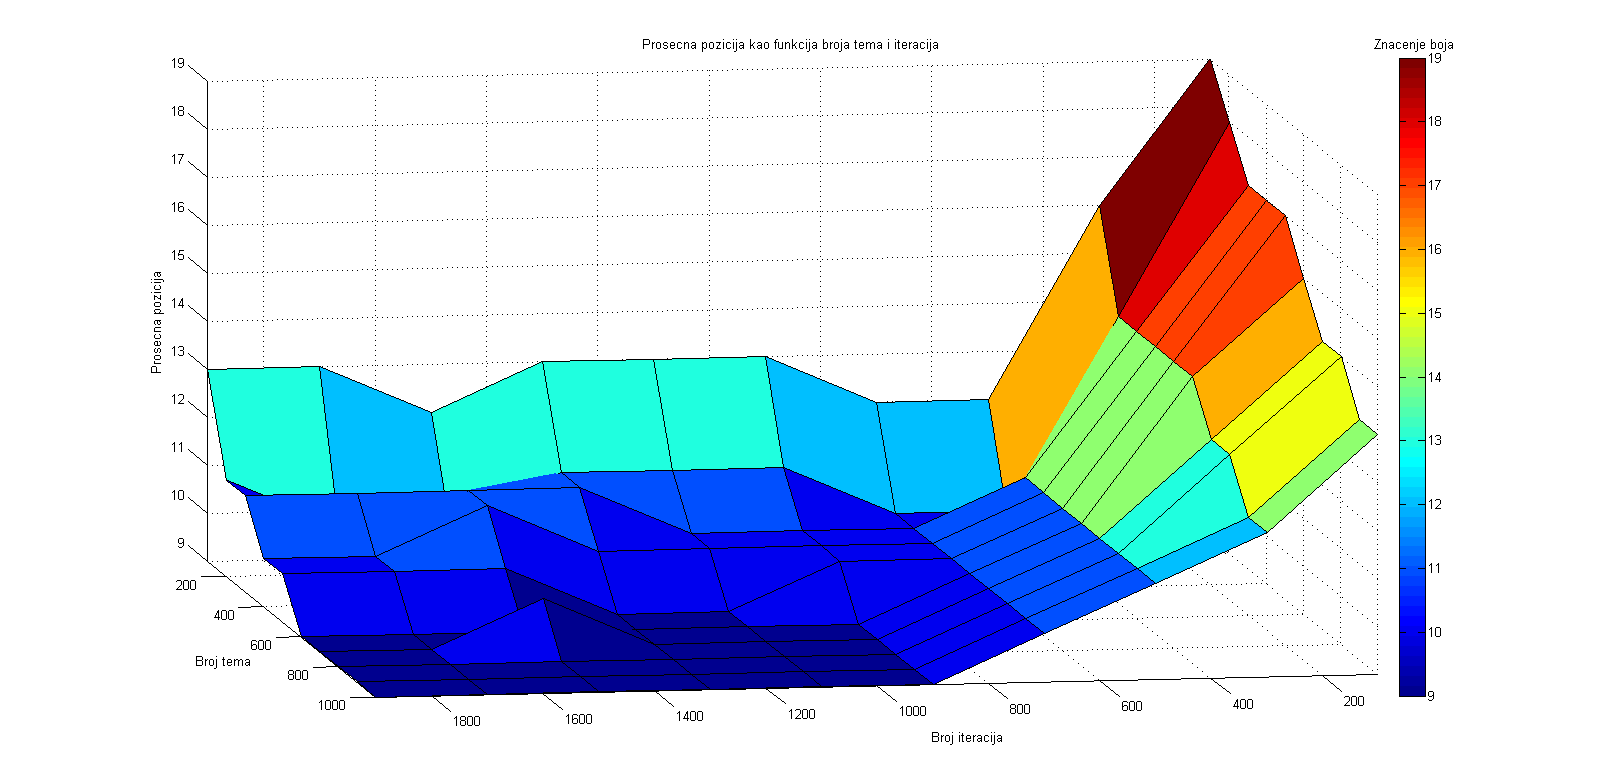
\includegraphics[scale=0.3]{./Slike/distnoStemNoSyn.png} 
	\caption{Зависност просечне позиције од броја тема и броја итерација}
	\label{fig:slika1}
\end{figure}

Минимална просечна позиција је \textbf{9} и добија се при више различитих комбинација параметара. Неке од комбинација су приказане у следећој табели

\begin{center}
\captionof{table}{Утицај броја тема и итерација на просечну позицију тачног одговора}
\begin{tabular}{|c|c|}
\hline
Број итерација & Број тема \\
\hline\hline
900 & 600 \\
900 & 700 \\
1100 & 500 \\
\hline
\end{tabular}

\end{center}


\subsection{Утицај стеминга на резултат}

Поред основне три трансформације, на улазне податке је примењене и стеминг модификација - уклњање наставака речи. Овим је полазни скуп података упрошћен јер је скуп различитих речи мањи. Без ове трансформације, једна иста реч у различитим родовима или временима се посматрала ралзличито што је довело до великог диверзитета у скупу речи ( на пример речи енг. think и енг. thinking су посматране као различите речи без обзира на исто основно значење речи ). 

\subsubsection{Косинусна сличност}



Утицај стеминга на просечну позицију  када се сличност мери косинусном сличношћу дат је на следећем графику( слика 5.2)

		\begin{figure}[H]
    \centering
   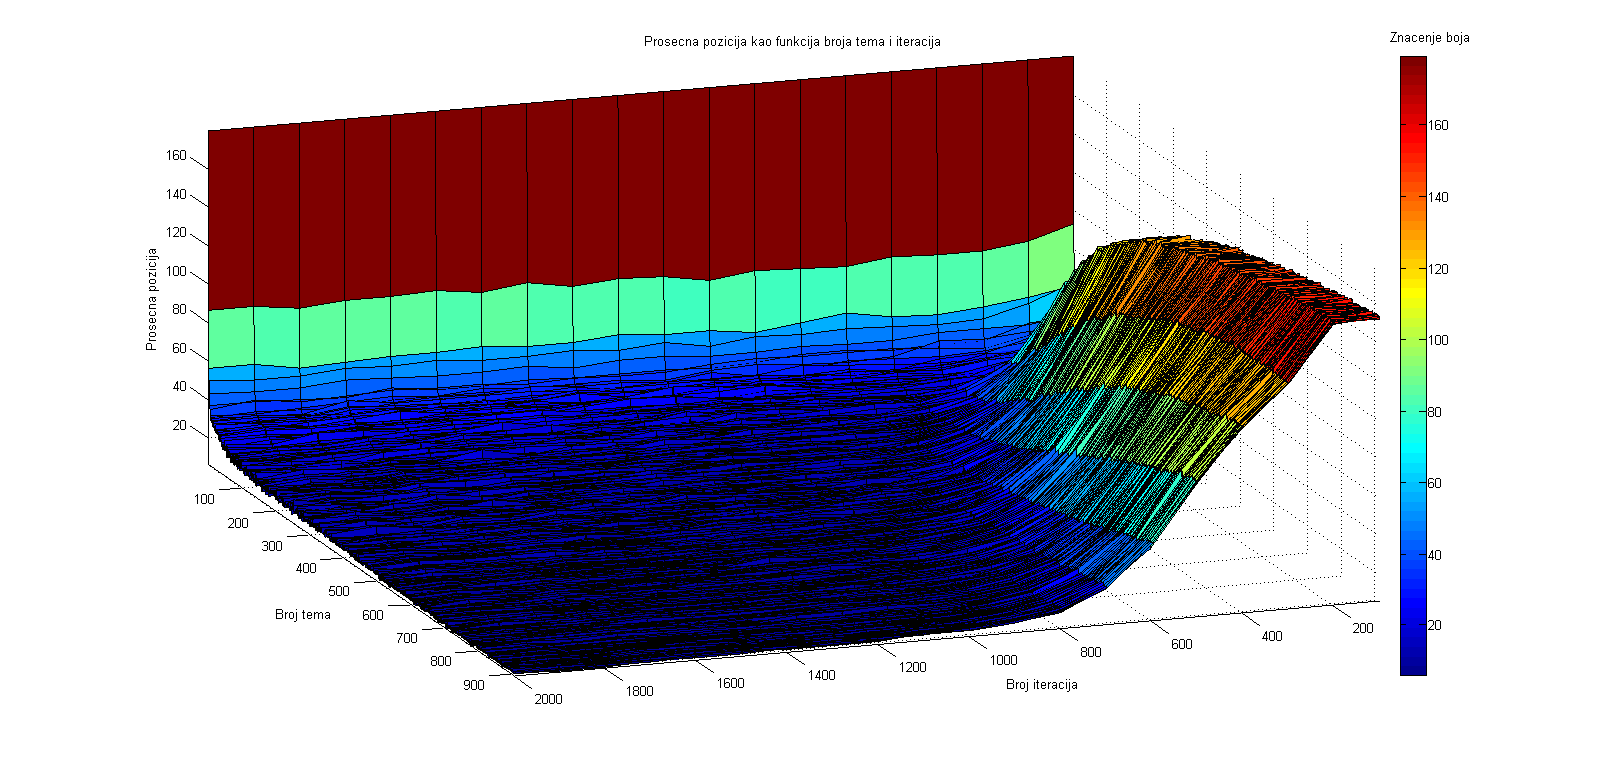
\includegraphics[scale=0.3]{./Slike/StemNoSyn.png} 
	\caption{Зависност просечне позиције од броја тема и броја итерација}
	\label{fig:slika1}
\end{figure}

Минимална просечна позиција је \textbf{6} и добија се при више различитих комбинација параметара. Неке од комбинација су приказане у следећој табели

\begin{center}
\captionof{table}{Утицај броја тема и итерација на просечну позицију тачног одговора}
\begin{tabular}{|c|c|}
\hline
Број итерација & Број тема \\
\hline\hline
1100 & 621 \\
1200 & 643 \\
1300 & 724 \\
\hline
\end{tabular}
\end{center}

Додавање стеминга утиче на нижу просечну позицију и на упрошћавање модела. Без примене стеминга, најједноставнији модел којим се постиже оптимална просечна позиција је био комбинација 1200 - 693 док је са стемингом то 1100 - 621. Дакле, додавањем и стеминга коришћењем мањег броја тема и у мање итерација постижу се бољи резултати. 


\subsubsection{Мерење сличности према лексичкој и тематској сличности}
	
Уколико се за меру сличности одабере мера  \textbf{лексичке и теметске} сличности, просечна позиција такође директно зависи од параметра модела. Обзиром на временску и просторну сложеност ове мере, нису испитиване све могућности за параметре модела. График зависности просечне позиције од броја тема и итерација дат јена следећој слици (слика 5.2)

		\begin{figure}[H]
    \centering
   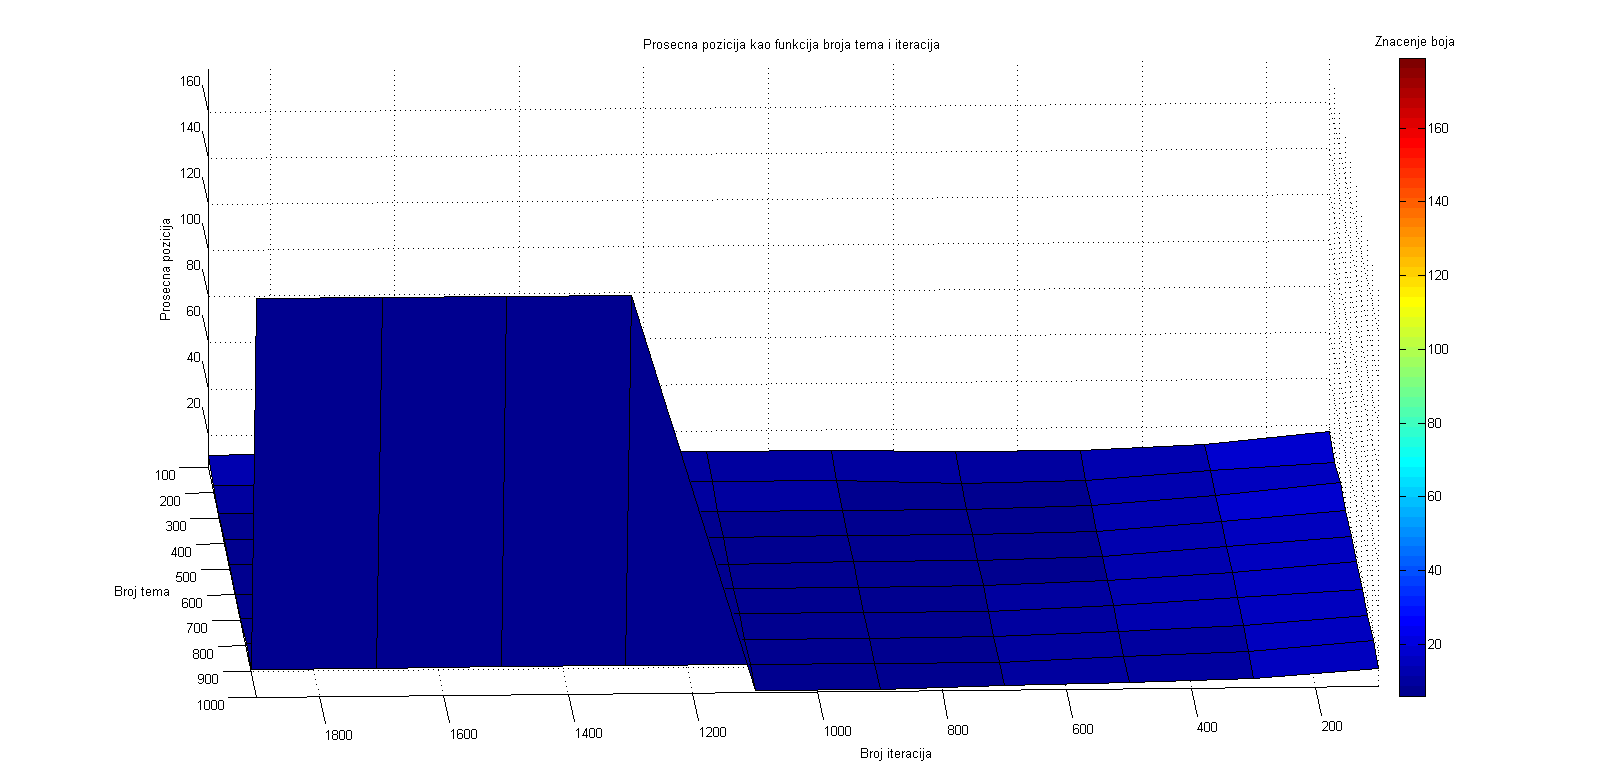
\includegraphics[scale=0.3]{./Slike/distStemNoSyn.png} 
	\caption{Зависност просечне позиције од броја тема и броја итерација}
	\label{fig:slika1}
\end{figure}

Минимална просечна позиција је \textbf{6} и добија се при више различитих комбинација параметара. Неке од комбинација су приказане у следећој табели

\begin{center}
\captionof{table}{Утицај броја тема и итерација на просечну позицију тачног одговора}
\begin{tabular}{|c|c|}
\hline
Број итерација & Број тема \\
\hline\hline
1100 & 500 \\
1300 & 600 \\
1300 & 800 \\
\hline
\end{tabular}

\end{center}


\subsection{Утицај лемитизације на резултат}

Лемитизација је процес свођења речи на \textbf{коренску} реч. Склањањем наставака речи могуће је пронаћи заједничку основу речи. Али, уколико реч мења облик у различитим лицима или временима, склањањем наставка речи, уколико уопше постоје, неће се добити иста реч. Лемитизацијом се овај проблем решева. На основу граматичких правила, препознаје се који основни облик реч и тим обликом замњује сепојављивање те речи у било којој форми. 




\subsubsection{Косинусна сличност}



Утицај лемитизације на просечну позицију  када се сличност мери косинусном сличношћу дат је на следећем графику( слика 5.2)

		\begin{figure}[H]
    \centering
   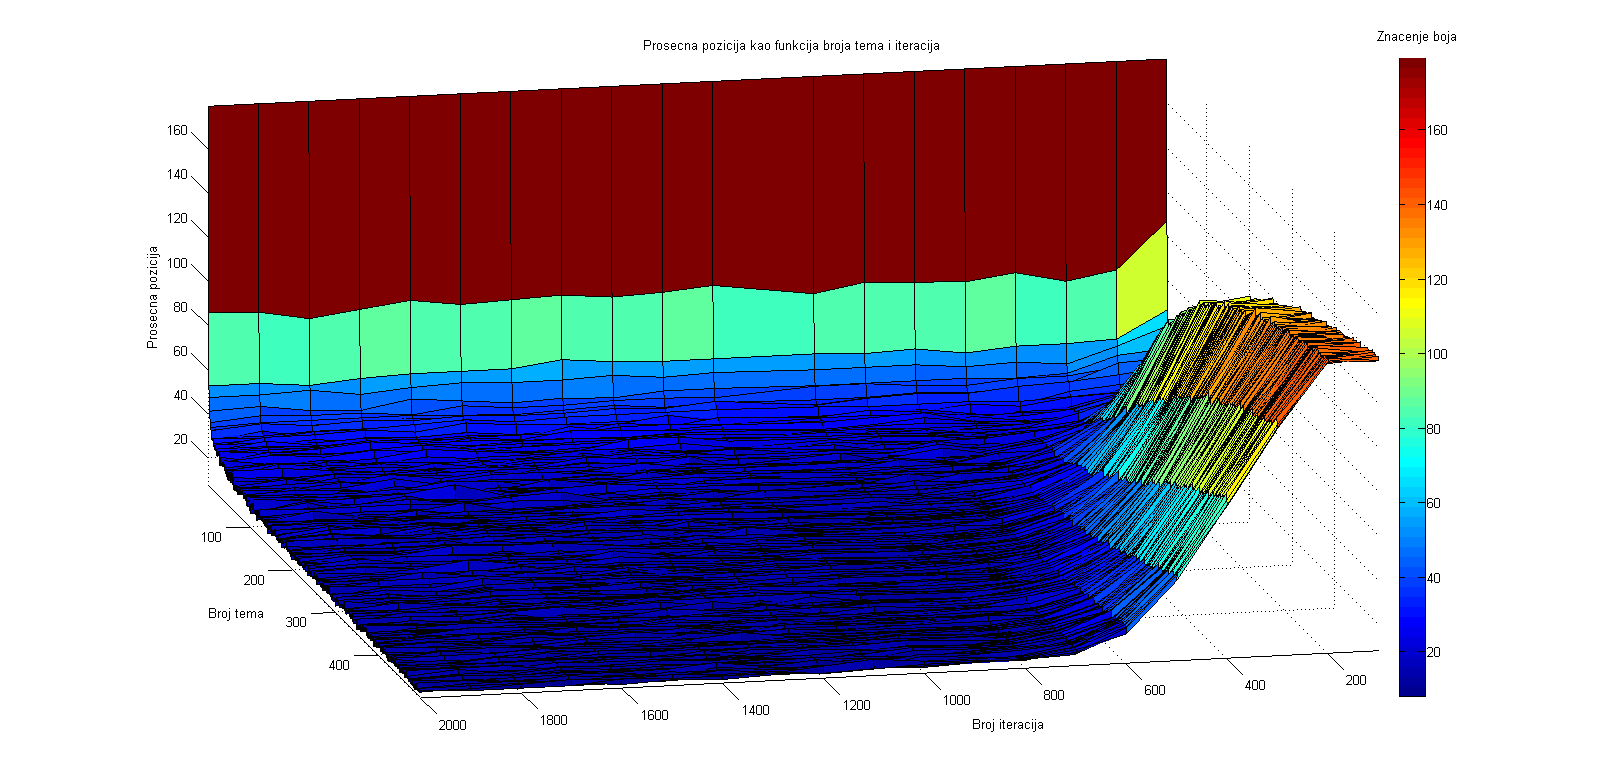
\includegraphics[scale=0.3]{./Slike/LemmNoSyn.png} 
	\caption{Зависност просечне позиције од броја тема и броја итерација}
	\label{fig:slika1}
\end{figure}

Минимална просечна позиција је \textbf{8} и добија се при више различитих комбинација параметара. Неке од комбинација су приказане у следећој табели

\begin{center}
\captionof{table}{Утицај броја тема и итерација на просечну позицију тачног одговора}
\begin{tabular}{|c|c|}
\hline
Број итерација & Број тема \\
\hline\hline
1300 & 481 \\
1300 & 486 \\
1500 & 481 \\
1600 & 477 \\
\hline
\end{tabular}
\end{center}

Може се закључити да лемитизација значајно утиче на поједностављивање модела. Најмања вредност просечне позције добије се коришћењем броја тема око  470 за разлику од основног модела где тај број износи преко 600.

Обзиром на то да лемитизација своди на коренску реч, мањи је диверзит скупа речи. Самим тим, моделу је теже да препозна прави одговор па је због тога просечна позиција више него просечна позиција која се добија употребом стеминга.



\subsubsection{Мерење сличности према лексичкој и тематској сличности}
	
Уколико се за меру сличности одабере мера  \textbf{лексичке и теметске} сличности, просечна позиција такође директно зависи од параметра модела. Обзиром на временску и просторну сложеност ове мере, нису испитиване све могућности за параметре модела. График зависности просечне позиције од броја тема и итерација дат јена следећој слици (слика 5.2)

		\begin{figure}[H]
    \centering
   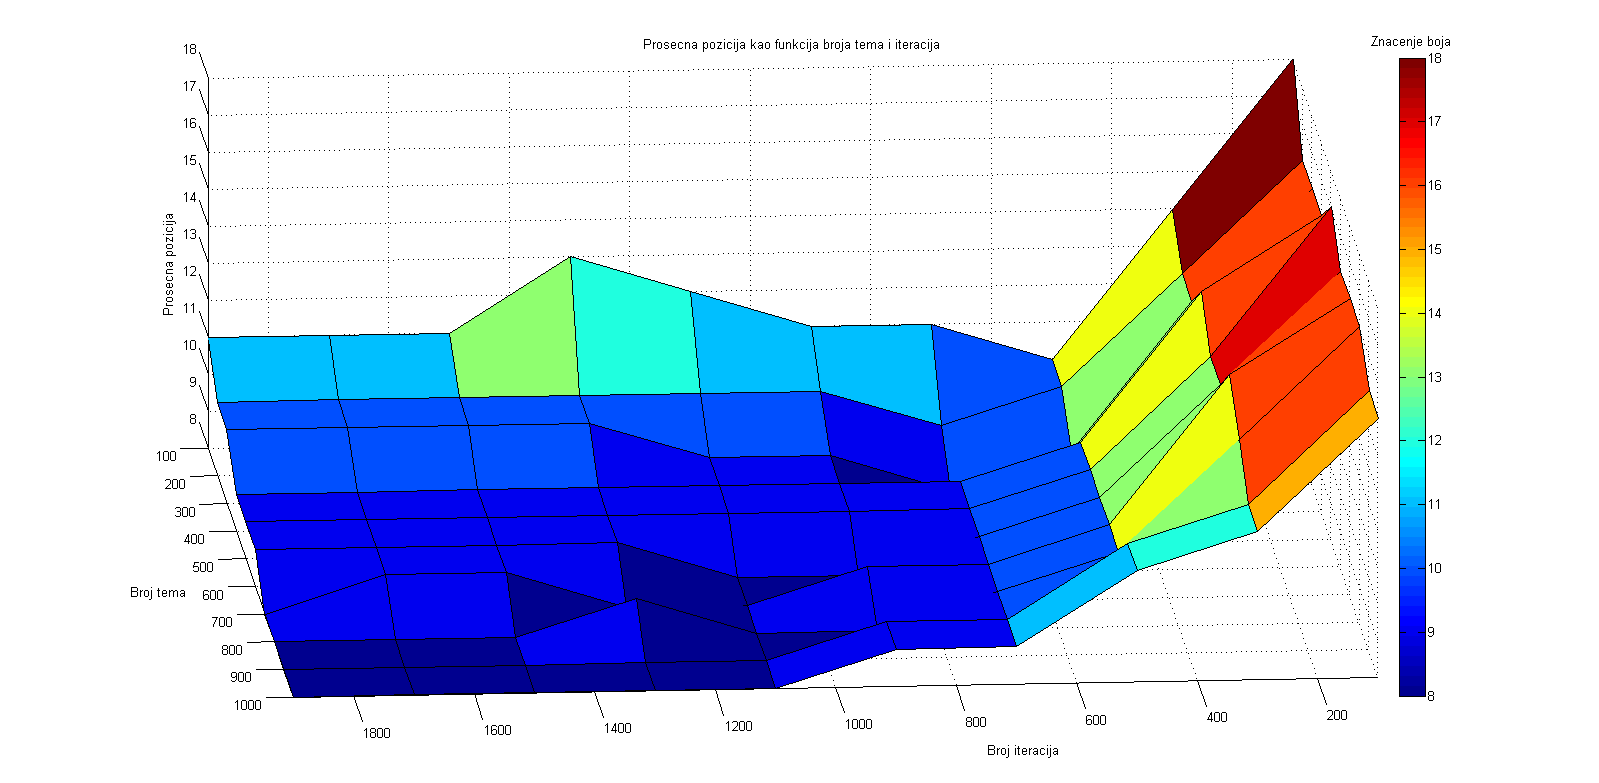
\includegraphics[scale=0.3]{./Slike/distLemNoSyn.png} 
	\caption{Зависност просечне позиције од броја тема и броја итерација}
	\label{fig:slika1}
\end{figure}

Минимална просечна позиција је \textbf{8} и добија се при више различитих комбинација параметара. Неке од комбинација су приказане у следећој табели

\begin{center}
\captionof{table}{Утицај броја тема и итерација на просечну позицију тачног одговора}
\begin{tabular}{|c|c|}
\hline
Број итерација & Број тема \\
\hline\hline
700 & 300 \\
900 & 600 \\
900 & 800 \\
\hline
\end{tabular}

\end{center}




\subsection{Утицај додавања синонима на резултат}

Додавање синонима речи има за циљ боље тематско одвајање. Наиме, уколико се свакој речи придода неколико синонима, претпоставља се да ће теметско одвајање бити једноставније. Основни разлог за увођење ове врсте трансформација била чињеница да  човек поузданије закључује "`о чему се ради"' у неком тексту уколико му се наведе неколико синонима за кључне речи. Обзиром да се ниједна реч не потенцира свакој речи је додат неки број синонима. Будући да додавање синонима директно утиче на перформансе система, у конкретном раду је одлучено да тај број буде 5.

 


\subsubsection{Косинусна сличност}



Утицај  на додавања синонима на просечну позицију  када се сличност мери косинусном сличношћу дат је на следећем графику( слика 5.2)

		\begin{figure}[H]
    \centering
   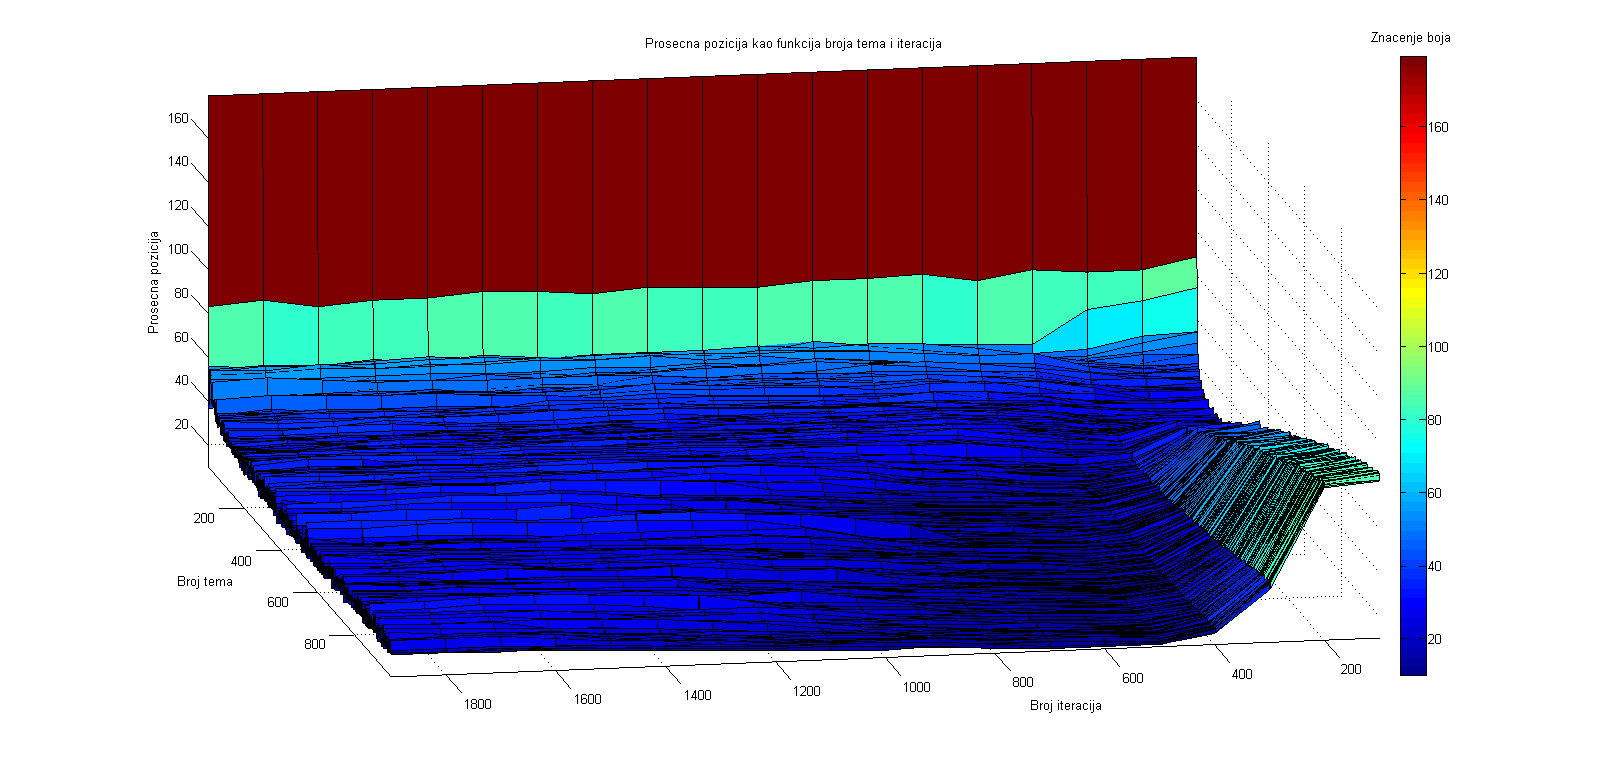
\includegraphics[scale=0.3]{./Slike/NoStemmSyn.png} 
	\caption{Зависност просечне позиције од броја тема и броја итерација}
	\label{fig:slika1}
\end{figure}

Минимална просечна позиција је \textbf{10} и добија се при више различитих комбинација параметара. Неке од комбинација су приказане у следећој табели

\begin{center}
\captionof{table}{Утицај броја тема и итерација на просечну позицију тачног одговора}
\begin{tabular}{|c|c|}
\hline
Број итерација & Број тема \\
\hline\hline
500 & 674 \\
500 & 675 \\
600 & 773 \\
500 & 991 \\
\hline
\end{tabular}
\end{center}

На основу облика графика може се закључити да додавање синонима утиче на екстремне вредности просечне позиције. Такође, упрошћава се модел и у мањем броју итреације достиже се минимална вредност просечне позиције. 
Са друге стране, пуно речи имају другачије значење у различитим контекстима а обзиром да у систем није убачено никакво додатно знање, постоји опасност од додавања неадекватних речи. То може да се одрази да немогућност прецизног одређивања тематске слике документа па и на прецизност решења.




\subsubsection{Мерење сличности према лексичкој и тематској сличности}
	
Уколико се за меру сличности одабере мера  \textbf{лексичке и теметске} сличности, просечна позиција такође директно зависи од параметра модела. Обзиром на временску и просторну сложеност ове мере, нису испитиване све могућности за параметре модела. График зависности просечне позиције од броја тема и итерација дат јена следећој слици (слика 5.2)

		\begin{figure}[H]
    \centering
   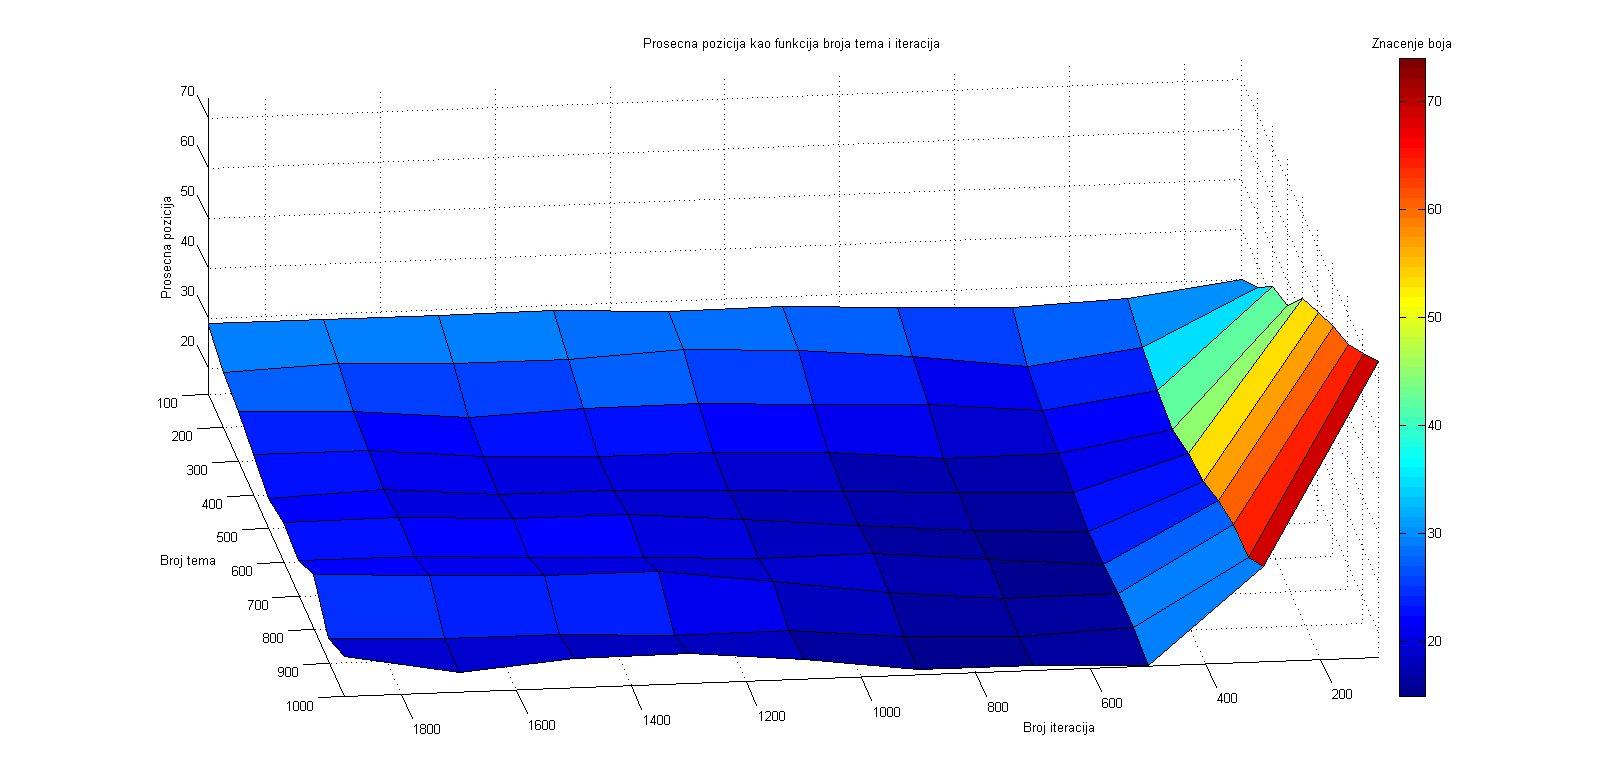
\includegraphics[scale=0.3]{./Slike/distNoStemSyn.png} 
	\caption{Зависност просечне позиције од броја тема и броја итерација}
	\label{fig:slika1}
\end{figure}

Минимална просечна позиција је \textbf{15} и добија се при више различитих комбинација параметара. Неке од комбинација су приказане у следећој табели

\begin{center}
\captionof{table}{Утицај броја тема и итерација на просечну позицију тачног одговора}
\begin{tabular}{|c|c|}
\hline
Број итерација & Број тема \\
\hline\hline
500 & 600 \\
500 & 700 \\
500 & 1000 \\
\hline
\end{tabular}

\end{center}





\subsection{Укупни резултати са синонимима и стемингом}

Поред поједничане примене сваке трансформације на улазне податке, у раду су тестиране и њихове комбинације. Обзором на то да стеминг уклања наставке, велики број тако модификованих добија нерегуларни облик. Због тога није могуће ни пронаћи њихове синониме. Да би се то избегло, најпре су додавани синоними за сваку реч а затим је извршен стеминг.

\subsubsection{Косинусна сличност}



Утицај  комбинације додавања синонима и стеминга на просечну позицију  када се сличност мери косинусном сличношћу дат је на следећем графику( слика 5.2)

		\begin{figure}[H]
    \centering
   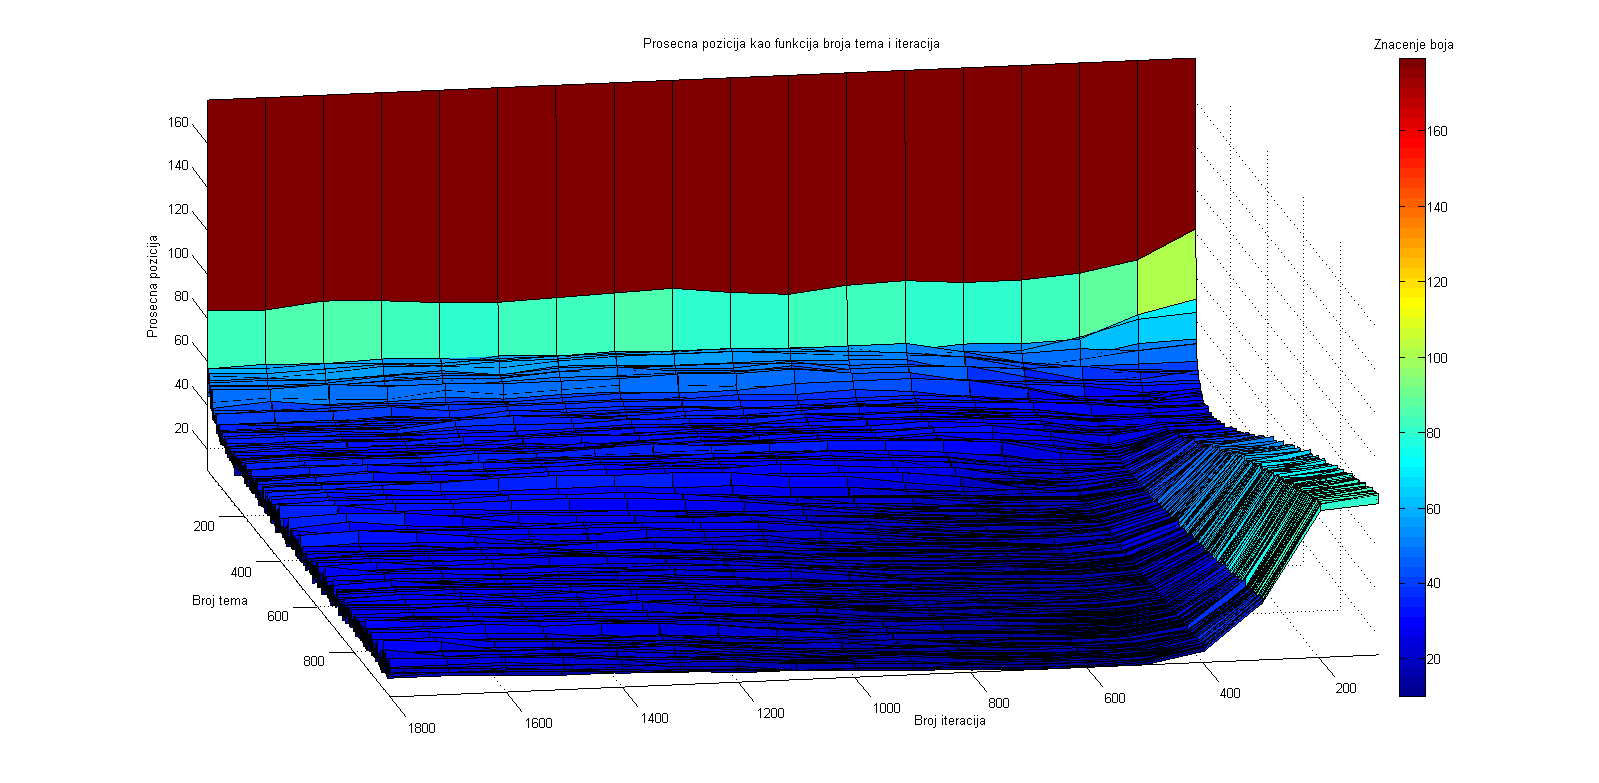
\includegraphics[scale=0.3]{./Slike/StemmSyn.png} 
	\caption{Зависност просечне позиције од броја тема и броја итерација}
	\label{fig:slika1}
\end{figure}

Минимална просечна позиција је \textbf{10} и добија се при више различитих комбинација параметара. Неке од комбинација су приказане у следећој табели

\begin{center}
\captionof{table}{Утицај броја тема и итерација на просечну позицију тачног одговора}
\begin{tabular}{|c|c|}
\hline
Број итерација & Број тема \\
\hline\hline
500 & 555 \\
500 & 690 \\
500 & 712 \\
700 & 847 \\
\hline
\end{tabular}
\end{center}

Са графика је јасно да је утицај синонима значајан. Облик површи је јако сличан облику који се добија додавањем само синонима, без примене стеминга. Дакле, додавање синонима има јачи утицај од стеминга. Односно, додавање стеминг трансформације након убацивања синонима не утиче значајно на просечну позицију. 

\subsection{Укупни резултати са синонимима и лемитизацијом}

Још једна од комбинација улазних трансформација која је тестирана у овом раду је и комбинација лемитизација и синоними. Лемитизација ће свести речи на коренску, без обзира на облик те речи. Међутим, поред означавања времена и лица, различит облик речи може означавати и различито значење речи. Из тог разлога, најпре су додати синоними па је затим примењена лемитизација.

\subsubsection{Косинусна сличност}



Утицај  комбинације додавања синонима и лемитизације на просечну позицију  када се сличност мери косинусном сличношћу дат је на следећем графику( слика 5.2)


		\begin{figure}[H]
    \centering
   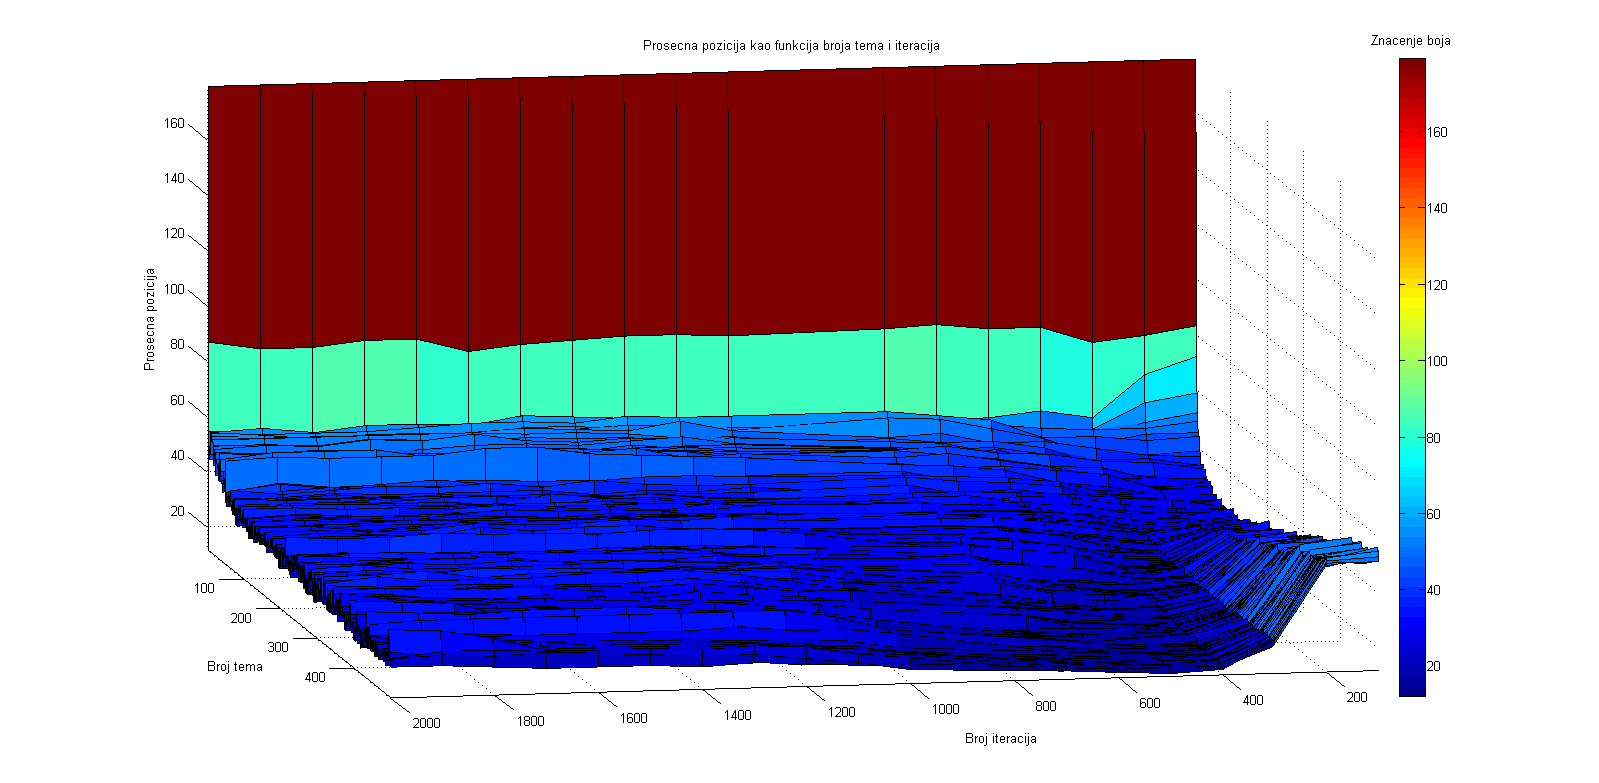
\includegraphics[scale=0.3]{./Slike/LemmSyn.png} 
	\caption{Зависност просечне позиције од броја тема и броја итерација}
	\label{fig:slika1}
\end{figure}

Минимална просечна позиција је \textbf{12} и добија се при тачно једној комбинацији параметара и то :

\begin{center}
\captionof{table}{Утицај броја тема и итерација на просечну позицију тачног одговора}
\begin{tabular}{|c|c|}
\hline
Број итерација & Број тема \\
\hline\hline
600 & 483 \\

\hline
\end{tabular}
\end{center}

Поново се примећује знатан утицај синонима на облик површи као и на просечну позицију. Лемитизација није значајно утицала на просечну позицију.



\subsubsection{Мерење сличности према лексичкој и тематској сличности}
	
Уколико се за меру сличности одабере мера  \textbf{лексичке и теметске} сличности, просечна позиција такође директно зависи од параметра модела. Обзиром на временску и просторну сложеност ове мере, нису испитиване све могућности за параметре модела. График зависности просечне позиције од броја тема и итерација дат јена следећој слици (слика 5.2)

		\begin{figure}[H]
    \centering
   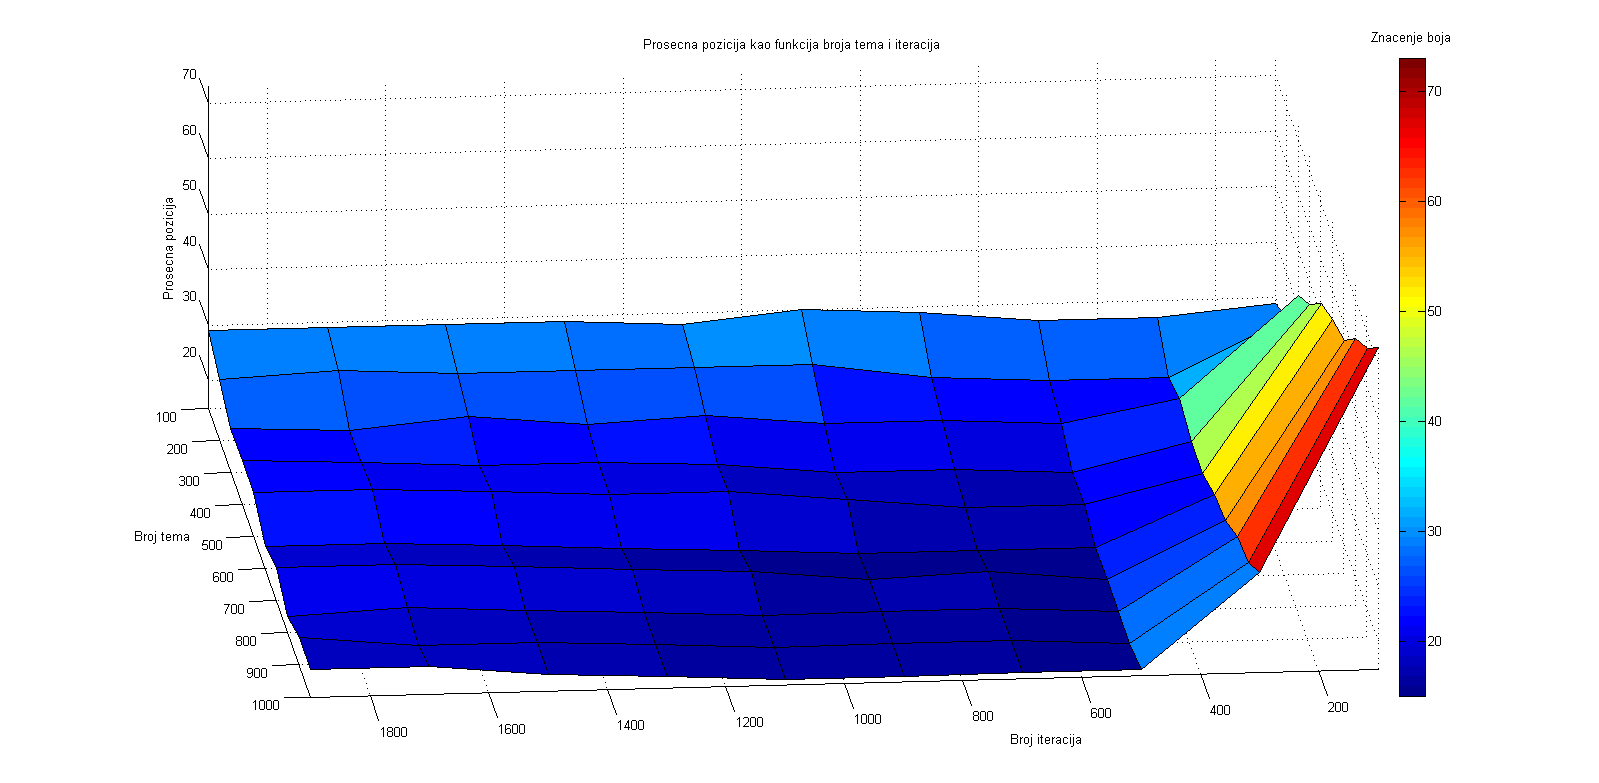
\includegraphics[scale=0.3]{./Slike/distLemmSyn.png} 
	\caption{Зависност просечне позиције од броја тема и броја итерација}
	\label{fig:slika1}
\end{figure}

Минимална просечна позиција је \textbf{15} и добија се при више различитих комбинација параметара. Неке од комбинација су приказане у следећој табели

\begin{center}
\captionof{table}{Утицај броја тема и итерација на просечну позицију тачног одговора}
\begin{tabular}{|c|c|}
\hline
Број итерација & Број тема \\
\hline\hline
500 & 600 \\
500 & 700 \\
500 & 800 \\
\hline
\end{tabular}

\end{center}




\section{Упоредни резултати решења алгоритмом моделовања тема и бројањем речи}




\subsection{Косинусна сличност}

\begin{center}
\captionof{table}{Упоредни резултати алгоритме моделовања тема и решења бројањем речи}
\begin{tabular}{ | l | l | l | l | l || l | l | l | l | }
\hline
	 &\multicolumn{4}{|c||}{WC}  & \multicolumn{4}{|c|}{TM}  \\ \hline
	 & Prva & Top 10 & Top 20 & Top 30 & Prva & Top 10 & Top 20 & Top 30 \\ \hline
	noStemNoSyn & 231 & 324 & 339 & 343 & 179 & 288 & 308 & 324 \\ \hline
	stemNoSyn & 233 & 331 & 345 & 350 & 190 & 296 & 319 & 330 \\ \hline
	lemmNoSyn & 231 & 333 & 345 & 350 & 187 & 297 & 329 & 336 \\ \hline
	stemSyn & 177 & 319 & 337 & 342 & 147 & 282 & 304 & 324 \\ \hline
	lemmSyn & 175 & 312 & 335 & 342 & 146 & 280 & 309 & 322 \\ \hline
	noStemSyn & 175 & 309 & 335 & 339 & 147 & 286 & 305 & 325 \\ \hline
\end{tabular}
\end{center}

Из резултата се може уочити да се косинусном мером расподела тема по документима не могу добити бољи резултати од класичног приступа бројањем речи. Разлог за то може да буде недовољна количина података али и природа мера сличности. Обзором да се узима само тематска сличност, занемарује се јако битна карактеристика сличности два документа - лексичка.

Добијени резултати, обзором да се ради о малом скупу података, могу да наведу на закључак да постоји извесна зависност између дужине питања( одговора) и датих решења. 



\subsection{Мерење сличности према лексичкој и тематској сличности}

Обзиром на то да је ова сличност јако велике сложености, из практичних разлога, нису тестиране све трансформације. Резултати који су добијени дати су у следећој табели:

\begin{center}
\captionof{table}{Упоредни резултати алгоритме моделовања тема и решења бројањем речи}
\begin{tabular}{ | l | l | l | l | l || l | l | l | l | }
\hline
	 &\multicolumn{4}{|c||}{WC}  & \multicolumn{4}{|c|}{TM}  \\ \hline
	 & 0 & 10 & 20 & 30 & 0 & 10 & 20 & 30 \\ \hline
	noStemNoSyn & 231 & 324 & 339 & 343 & 217 & 308 & 332 & 340 \\ \hline
	stemNoSyn & 233 & 331 & 345 & 350 & 215 & 325 & 339 & 343 \\ \hline
	lemmNoSynEnd & 231 & 333 & 345 & 350 & 213-232 & 319 & 338 & 342 \\ \hline
	lemmSyn & 175 & 312 & 335 & 342 & 150 & 270 & 288 & 304 \\ \hline
\end{tabular}
\end{center}


Дакле, ова мера показује незнатно слабије резултате од класичног метода, стим што јој је комплекснонст знатно већа. Са друге стране, добијена прецизност решења је већа него код косинусне сличности.Међутим, како је потребно доста времена да би се добили резултати, ова мера није даље разматрана. 

\subsection{Сличност према предвиђеној вероватноћи}

Полазни тестни скуп има 360 питања и 360 одговора. Он је довољно мали да омогућава тестирање сваке од поменутих мера, довољно велики да би се уочили трендови али недовољан да би се донели генерални закључци. 

Обзиром на то да је ова мера  показала најбоље резултате, поред стандардног тестног скупа, тестирана је и на већим скуповима података. Величине додатних скупова података су по 200, 800, 1400, 2000, 10000, 20000 и 40000 докумената, односно 100, 400, 700, 1000, 5000, 10000 и 20000 питања и исто толико одговора. Подаци су преузети са сајта \textit{answers.yahoo.com}

Ова додатна тестирања су била неопходна како би се избегао енг. overfitting, тј. како би се донели закључци који што мање зависе од података. 

Енг. overfitting је термин машинског учења који се односии на прилагођавање програма подацима. Тада се најчешће дешава да програм  са изузетно великом прецизношћу  ради са једним скупом података, док са другим скупом та прецизност драстично опада. Разлог томе је што је програм \textbf{научен} да ради само са одређеним скупом података .
У конкретном случају, немогуће је потпуно побећи од енг. overfitting-а због природе проблема. Међутим, уколико се покаже да модели грађени над различитим скупом података показују исте особине, тада се могу извести закључци који су релативно независни од података. 
 

Компаративни модел, као и досада било је решење бројањем речи. Резултати добијени мерењем дати су у следећој табели :
\begin{table}[H]
\centering
\caption{Упоредни резултати решења алгоритма моделовања тема употребом мере сличности на основу предвиђене вероватноће и компаративног решења}
\begin{tabular}{ | l | l | l | l | l || l | l | l | l | l | }
\hline
	 & \multicolumn{4}{|c||}{WC}  & \multicolumn{5}{|c|}{TM}  \\ \hline
	Broj dokumenata & Prva & Top 10 & Top 20 & Top 30 & Prva & Top 10 & Top 20 & Top 30 &  Br. tema \\ \hline
	100 & 72 & 90 & 91 & 91 & 66 & 87 & 91 & 94 & 50 \\ \hline
	400 & 203 & 338 & 353 & 361 & 217 & 326 & 336 & 348 & 400 \\ \hline
	700 & 338 & 569 & 596 & 610 & 357 & 546 & 583 & 594 & 750 \\ \hline
	1000 & 453 & 789 & 836 & 853 & 472 & 744 & 794 & 829 & 1100 \\ \hline
	5000 & 1484 & 3002 & 3367 & 3570 & 1614 & 2960 & 3279 & 3472 & 800 \\ \hline
	10000 & 2422 & 5334 & 6054 & 6521 & 2766 & 5297 & 5988 & 6421 & 1100 \\ \hline
	20000 & 3866 & 9044 & 10516 & 11460 & 4576 & 9182 & 10546 & 11358 & 900 \\ \hline
\end{tabular}
\end{table}

Као што се може приметити, алгоритам моделовања тема готово увек успева да на прву позицију избаци више тачних одговора него компаративно решење. Једино за  улазни скуп од 100 питања и 100 одговора ово није испуњено, иако не одступа много. Може бити више разлога за овакво понашање:
\begin{itemize}
\item Природа података које погодује компаративном решењу
\item Недовољна количина података - модел  нема довољно информација
\end{itemize}

Даље испитивање узрока оваквог понашања није од интереса. Пре свега, улазни скуп је јако мали, тако да резултати доста зависе од података. Са друге стране, ова величина скупа је недовољна за било какву реалну примену.

Уколико се графички представи број докумената који се појављују на првој позицију у односу на величину улазног скупа, може се приметити да са повећањем улазних података, разлика у резултатима ова два решења постаје већа. Графички приказ дат је на следећој слици :

\begin{figure}[H]
  \centering
   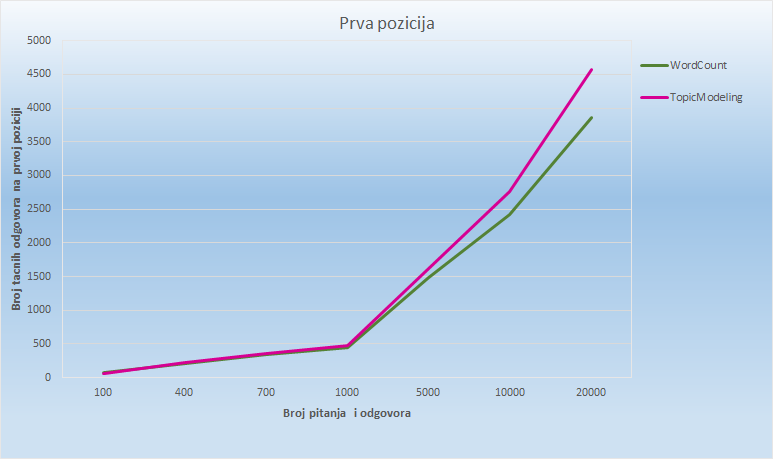
\includegraphics[scale=0.8]{./Slike/prvePoz.png} 
	\caption{Прва позиција у односу на величину улазног скупа}
	\label{fig:slika1}
\end{figure}

Појављивање тачног одговора на првој позицији може бити престрог критеријум за упоређивање резултате ове две методе. Стога се поред прве позиције, за меру оцене може узети и појављивање тачног одговора у првих 10 предложених резултата. Графички приказ резултата поменуте две методе дат је на следећој слици.

\begin{figure}[H]
  \centering
   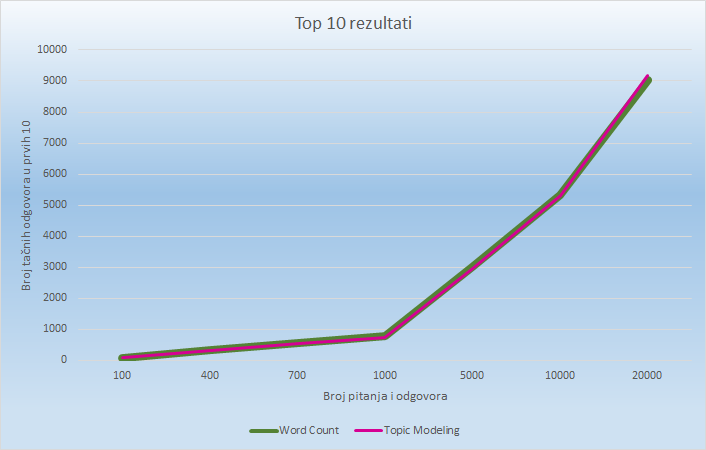
\includegraphics[scale=0.8]{./Slike/top10.png} 
	\caption{Број тачних одговора у првих 10 предложених резултата у односу на величину улазног скупа}
	\label{fig:slika1}
\end{figure}

Као што се може уочити са слике, резултати ове две методе мерене са становишта првих 10 предложених резултата, готово се идентично понашају. 



Поред броја тачнох одговора који се налазе на првој позицији, или у првих 10 предложених одговора, важна карактериста оба решења је \textbf{прецизност}. Под прецизношћу решења подразумева се \textbf{проценат} тачних одговора који испуњавају неки критеријум. У конкретном случају, од интереса је да ли се налазе на првој позицији, односно да ли се налазе у првих 10 предложених решења.

Прецизност оба решења у односу на то да ли се тачан одговор појављује на првој позицији у листи предложених одговора дат је на следећој слици :

\begin{figure}[H]
  \centering
   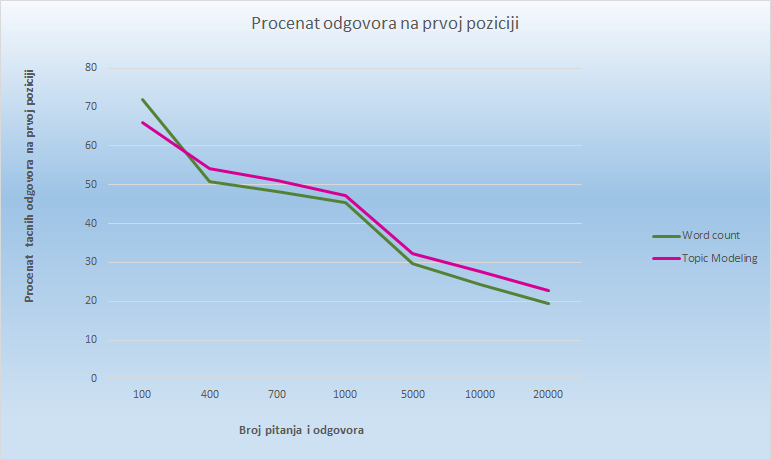
\includegraphics[scale=0.8]{./Slike/procenatPrva.png} 
	\caption{Прецизност предложених решења}
	\label{fig:slika1}
\end{figure}

Са слике се може закључити следеће :
\begin{itemize}
\item Оба решења губе прецизност са повећањем броја улазних података
\item Прецизност решења алгоритмом моделовања тема спорије опада него прецизност решења бројањем речи
\item Разлика у прецизности ова два решења повећава се са повећањем броја улазних података
\end{itemize}

Упоредна прецизност предложених решења у односу на то да ли се тачан одговор налази у првих 10 предложених одговора, дата је на следећем графику :

\begin{figure}[H]
  \centering
   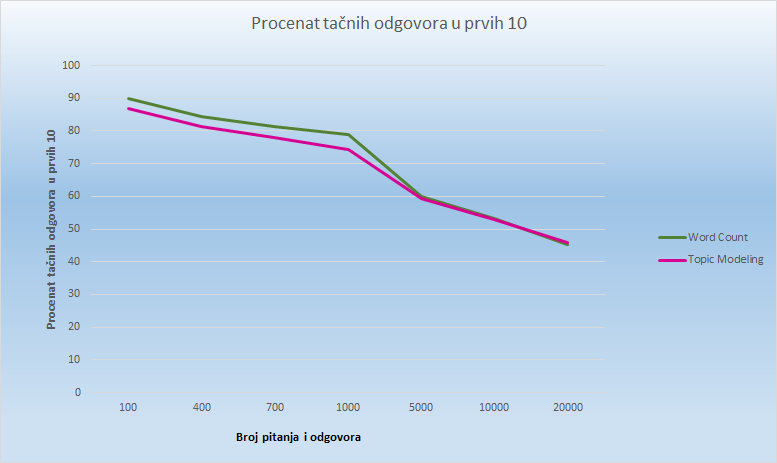
\includegraphics[scale=0.8]{./Slike/procenat10.png} 
	\caption{Прецизност предложених решења}
	\label{fig:slika1}
\end{figure}

Могу се извести слични закључци као и за прецизност везану за појављивање тачног одговора на првој позицији :

\begin{itemize}
\item Са порастом величине улазних података, прецизност оба решења опада
\item Прецизност решења бројањем речи је већа него прецизност решења моделовањем тема за величину улазнпог скупа до 5000. Након тога, прецизности оба решења су готово исте.
\end{itemize}


\textbf{Статистичка значајност разлике у резултатима}\\

Како би изведени закључци били поузданији, урађени су и статистички тестови значајности над добијеним резултатима. У конкретном случају рађен је Вилкоксонов тест за упоредне резултате добијене на првој позицији оба решења. Овим тестом се испитује  да ли постоји статистички значајна разлика у резултатима ове две методе. Услов значајности је да сигнификантност добијена овим тестом буде $<0.05$. Резултати тестова налазе се у следећој табели :
\begin{table}[H]
\centering
\caption{Резултати Вилкоксоновог теста}

\begin{tabular}{ | l | l | l | l | l | }
\hline
	
	Broj dokumenata & Prva WC & Prva TM & Signifikantnost & Značajno \\ \hline
	100 & 72 & 66 & 0.71099999999999997 & NE \\ \hline
	400 & 203 & 217 & 3.1E-2 & DA \\ \hline
	700 & 338 & 357 & 2.1000000000000001E-2 & DA \\ \hline
	1000 & 453 & 472 & 2E-3 & DA \\ \hline
	5000 & 1484 & 1614 & 7.4999999999999997E-2 & NE \\ \hline
	10000 & 2422 & 2766 & 2.7E-2 & DA \\ \hline
	20000 & 3866 & 4576 & 0 & DA \\ \hline
	
\end{tabular}

\end{table}

На основу резултата у претходној табели, може се закључити да разлике у мерењима нису случајне већ зависне од метода. При тестирању резултата на скупу од 5000 одговора, утврђено је да разлике између метода нису статистички значајне. Ово не мора да значи да разлике између метода не постоје. Праг значајности са којим су рађени тестови је 0.05, док је сигнификантност добијена у овом скупу података 0.07. Ова мала разлика може да буде последица од грешке у рачуну ( нагомилана грешка ) до специфичности података. 